



\chapter{Statistiques descriptives}

\arrayrulecolor{Couleur6}


\section{Caractéristiques d'une série statistique}

\subsection{Série statistique}
Voici les séries de notes obtenues par 3 élèves :
\begin{itemize}[label=\textbullet]
\item  Jérôme : $\quad 4 \quad; \quad 6 \quad; \quad 18 \quad; \quad 7 \quad; \quad 17 \quad ; \quad 12 \quad ; \quad 12 \quad ;\quad  18$
\item Bertrand : $\quad 13 \quad ; \quad 13\quad ; \quad 12 \quad ; \quad 10 \quad ; \quad 12 \quad ; \quad 3\quad ; \quad 14 \quad ; \quad 12 \quad ; \quad 14 \quad ; \quad 15$
\item  Julie: $\quad 15 \quad ; \quad 9 \quad ; \quad 14 \quad ; \quad 13 \quad ; \quad 10 \quad ; \quad 12 \quad ; \quad 12 \quad ; \quad 11 \quad ; \quad 10$
\end{itemize}

\subsection{Moyenne}

Calculer la moyenne pour chaque série de notes de Jérôme, de Bertrand et de Julie.

 $$\text{M}_{(\text{Jérôme})} =\dfrac{4+6+18+7+17+12+12+18}{8}\approx 11,8$$
 $$\text{M}_{(\text{Bertrand})} =\dfrac{13+13+12+10+12+3+14+12+14+15}{10}=11,8 $$
 $$\text{M}_{(\text{Julie})} =\dfrac{15+9+14+13+10+12+12+11+10}{9}\approx 11,8$$


Une autre manière de calculer la moyenne est d'utiliser la moyenne pondérée : 

\begin{Définition}

La {\bf{moyenne}} d'une série statistique dont les valeurs sont $x_1, x_2 , ..., x_k$ et les effectifs correspondants $n_1$, $n_2$, ..., $n_k$ est notée $\overline{x}$ et est égale à : $$ \overline{x} = \dfrac{n_1x_1 + n_2x_2 + \cdots +n_kx_k}{n_1+n_2+\cdots +n_k}$$\\
La {\bf{moyenne}} est une caractéristique de position.
\end{Définition} 

\begin{Méthode}
$ \\
 $Il faut d'abord ranger les valeurs dans l'ordre croissant. \\
Dans notre exemple, on a :
 $$\text{M}_{(\text{Jérôme})} =\dfrac{4+6+7+2\times 12+17+2\times 18}{8}\approx 11,8$$
$$\text{M}_{(\text{Bertrand})} =\dfrac{3 + 10 +3\times 12 + 2 \times 13+2\times 14+15}{10}=11,8 $$
$$\text{M}_{(\text{Julie})} =\dfrac{9 + 2\times 10 +11+2\times 12+13 +14+15}{9}\approx 11,8$$

\end{Méthode}


\newpage

\subsection{Médiane}

\begin{Définition}
La {\bf{médiane}} $Me$ est une valeur telle que la moitié au moins de l'effectif ait des valeurs inférieures ou égales à $Me$, l'autre moitié des valeurs supérieures ou égales à $Me$.\\
La {\bf{médiane}} est une caractéristique de position.
\end{Définition}

\begin{Méthode}
Pour déterminer les notes médianes, il faut ordonner les séries. \\
 La médiane partage l'effectif en deux. \\
Calculer la médiane pour chaque série de notes de Jérôme, de Bertrand et de Julie. \\


\textbf{Jérôme :} 

\begin{center}
$\underbrace{4 ~ ~ 6 ~~ 7 ~~ \textcolor{Couleur8}{12}}_{4 \text{ données}} \quad \underbrace{\textcolor{Couleur8}{12} ~~ 17 ~~ 18 ~~ 18}_{4 \text{ données}}$
\end{center}

$\text{Donc } Me_{(\text{Jérôme})}=\textcolor{Couleur8}{12}$ \\[1em]

\textbf{Bertrand :} 

\begin{center}
$\underbrace{3 ~ ~ 10 ~~ 12 ~~ 12 ~~\textcolor{Couleur8}{12}}_{5 \text{ données}} \quad \underbrace{\textcolor{Couleur3}{13} ~~ 13 ~~ 14 ~~ 14 ~~15}_{5 \text{ données}}$
\end{center}

$\text{Donc } Me_{(\text{Bertrand})}=\dfrac{\textcolor{Couleur8}{12}+\textcolor{Couleur3}{13}}{2}=12,5$\\[1em]

\textbf{Julie :} 

\begin{center}
$\underbrace{9 ~ ~ 10 ~~ 10 ~~ 11}_{4 \text{ données}} \quad \textcolor{Couleur7}{\textbf{12}} \quad \underbrace{12 ~~ 13 ~~ 14 ~~15}_{4 \text{ données}}$
\end{center}

$\text{Donc } Me_{(\text{Julie})}=\textcolor{Couleur7}{\textbf{12}}$
\end{Méthode}

\subsection{Étendue}

\begin{Définition}
L'{\bf{étendue}} d'une série statistique est la différence entre la plus grande valeur et la plus petite valeur de la série. \\
L'{\bf{étendue}} est une caractéristique de dispersion.

\end{Définition}

\noindent Calculer l'étendue pour chaque série de notes de Jérôme, de Bertrand et de Julie.

\begin{multicols}{3}
\begin{itemize}[label=\textbullet]
\item  $\text{E}_{(\text{Jérôme})} =18-4=14$
\item $\text{E}_{(\text{Bertrand})} =15-3=12 $
\item $\text{M}_{(\text{Julie})} =15-9=6$
\end{itemize}
\end{multicols}

La note minimale de Bertrand est $3$ pourtant, cela ne représente pas vraiment la série de notes de Bertrand. 



\begin{Remarque}
Conclusion : l'étendue est un paramètre de dispersion absolue qui est simple à calculer mais très fragile puisqu'il ne dépend que de deux valeurs de la distribution. Ce paramètre n'a guère de signification lorsqu'une distribution comporte des valeurs exceptionnelles. 
\end{Remarque}

\newpage

\subsection{Quartiles, écart interquartile}
\begin{Définition}
Le {\bf{premier quartile}}  $(Q_1)$ est la plus petite valeur de la série telle qu'au moins $25 \%$ des autres valeurs de la série sont inférieures ou égales à cette valeur.\\
Le  {\bf{troisième quartile}} $(Q_3)$ est la plus petite valeur de la série telle qu'au moins $75 \%$ des autres valeurs de la série sont inférieures ou égales à cette valeur.\\
Les {\bf{quartiles}} sont des caractéristiques de position.

\end{Définition}

\begin{Définition}
L'{\bf{écart interquartile}} d'une série statistique de premier quartile $Q_1$ et de troisième quartile $Q_3$ est égal \\ à la différence $Q_3 - Q_1$. \\
L'{\bf{écart interquartile}} est une caractéristique de dispersion.


\end{Définition}
\vspace{0.3cm}
\begin{Remarque}
L'écart interquartile d'une série mesure la dispersion autour de la médiane. Il contient au moins $50\%$ des valeurs de la série.
L'écart interquartile n'est pas influencé par les valeurs extrêmes de la série.
\end{Remarque}
\vspace{0.3cm}
\begin{Méthode}
Calculer les quartiles pour chaque série de notes de Jérôme de Bertrand et de Julie.\\
Pour déterminer les quartiles, il faut ordonner les séries.\\
Le premier quartile est la donnée de la série se trouvant au quart de l'effectif.\\
Le troisième quartile est la donnée de la série se trouvant au trois-quarts de l'effectif.\\

\textbf{Jérôme :} ~~~~
$ 4 ~ ~ \textcolor{Couleur8}{6} ~~ 7 ~~ 12 ~~ 12 ~~ \textcolor{Couleur3}{17} ~~ 18 ~~ 18 $\\[0.5em]
$ \dfrac{1}{4}\times 8=2 $ le premier quartile est la \textcolor{Couleur8}{2e donnée} de la série.\\[0.5em]
$ \dfrac{3}{4}\times 8=6 $ le troisième quartile est la \textcolor{Couleur3}{6e donnée} de la série.\\[0.5em]
$ Q_{1(\text{Jérôme})} = 6 $ et $ Q_{3(\text{Jérôme})} = 17 $\\
L'écart interquartile est égale à $ E_{Q(\text{Jérôme})}= Q_{3(\text{Jérôme})}-Q_{1(\text{Jérôme})}=17-6=11$
\\[1em]


\textbf{Bertrand :} 
$ 3 ~ ~ 10 ~~ \textcolor{Couleur8}{12} ~~ 12 ~~12 ~~ 13 ~~ 13 ~~ \textcolor{Couleur3}{14} ~~ 14 ~~15 $\\[0.5em]
$ \dfrac{1}{4}\times 10=2,5 $ le premier quartile est la \textcolor{Couleur8}{3e donnée} de la série.\\[0.5em]
$ \dfrac{3}{4}\times 10=7,5 $ le troisième quartile est la \textcolor{Couleur3}{8e donnée} de la série.\\[0.5em]
$ Q_{1(\text{Bertrand})} = 12 $ et $ Q_{3(\text{Bertrand})} = 14 $\\
L'écart interquartile est égale à $ E_{Q(\text{Bertrand})}= Q_{3(\text{Bertrand})}-Q_{1(\text{Bertrand})}=14-12=2$\\[1em]



\textbf{Julie :} 
$ 9 ~ ~ 10 ~~ \textcolor{Couleur8}{10} ~~ 11 ~~12~~ 12 ~~ \textcolor{Couleur3}{13} ~~ 14 ~~15 $\\[0.5em]
$ \dfrac{1}{4}\times 9=2,25 $ le premier quartile est la \textcolor{Couleur8}{3e donnée} de la série.\\[0.5em]
$ \dfrac{3}{4}\times 9=6,75 $ le troisième quartile est la \textcolor{Couleur3}{7e donnée} de la série.\\[0.5em]
$ Q_{1(\text{Julie})} = 10 $ et $ Q_{3(\text{Julie})} = 13 $\\
L'écart interquartile est égale à $ E_{Q(\text{Julie})}= Q_{3(\text{Julie})}-Q_{1(\text{Julie})}=13-10=3$



\end{Méthode}

\newpage

\subsection{Interprétations}

\begin{center}
\begin{tabular}{|c|c|c|c|c|c|}
\hline
${\color{Couleur1}{\text{M}_{(\text{Jérôme})}\approx 11,8}}$ & ${\color{Couleur3}{\text{Me}_{(\text{Jérôme})}= 12}}$ &  ${\color{Couleur8}{\text{E}_{(\text{Jérôme})}=14}}$ & ${\text{Q}_1}_{(\text{Jérôme})}=6$ & ${\text{Q}_3}_{(\text{Jérôme})}=17$ & ${\color{Couleur7}{{\text{E}_Q}_{(\text{Jérôme})}=11}}$ \\
\hline
${\color{Couleur1}{\text{M}_{(\text{Bertrand})} =11,8}} $ & $\text{Me}_{(\text{Bertrand})} =12,5 $ & ${\color{Couleur8}{\text{E}_{(\text{Bertrand})} =12}} $ & ${\color{Couleur6}{{\text{Q}_1}_{(\text{Bertrand})} =12}} $& ${\text{Q}_3}_{(\text{Bertrand})} =14 $ &${\text{E}_Q}_{(\text{Bertrand})} =2 $  \\
\hline
${\color{Couleur1}{\text{M}_{(\text{Julie})} \approx 11,8}}$ & $\text{Me}_{(\text{Julie})} = 12$ &  ${\color{Couleur8}{\text{E}_{(\text{Julie})} = 6}}$ & ${\text{Q}_1}_{(\text{Julie})} = 10$ &  ${\color{Couleur6}{{\text{Q}_3}_{(\text{Julie})} = 13}}$ &  ${\text{E}_Q}_{(\text{Julie})} = 3$ \\
\hline
\end{tabular}
\end{center}

~\\
\noindent {\textcolor{Couleur1}{Les moyennes sont environ égales}} et pourtant {\textcolor{Couleur8}{les notes ne se répartissent pas de la même manière autour de cette caractéristique de position. Les étendues sont très différentes}}.\\
{\textcolor{Couleur3}{Jérôme à une médiane égale à $12$ donc il a obtenu autant de notes au-dessus de $12$ que de notes en-dessous de $12$.}}\\
{\textcolor{Couleur6}{Le premier quartile de Bertrand est égal à $12$ donc au moins un quart des notes de Bertrand sont inférieures à $12$.}}\\
{\textcolor{Couleur6}{Le troisième quartile de Julie est égal à $13$ donc au moins trois quarts des notes de Julie sont inférieures à $13$.}}\\
{\textcolor{Couleur7}{L'écart interquartile de Jérôme est égal à $11$ donc il a au moins $50\%$ des notes comprises entre $6$ et $17$ (les quartiles).}}

\begin{center}
\begin{tikzpicture}[scale=1.2]
    % Définition des positions (échelle arbitraire de 0 à 10)
    \def\min{0}
    \def\q{2.5}      % Q1 (25%)
    \def\med{5}      % Médiane (50%)
    \def\qtres{7.5}  % Q3 (75%)
    \def\max{10}     % Maximum
    
    % Boîte principale (de Q1 à Q3)
    \draw[thick] (\q,0.5) rectangle (\qtres,1.5);
    
    % Ligne de la médiane
    \draw[thick] (\med,0.5) -- (\med,1.5);
    
    % Moustaches (whiskers)
    \draw[thick] (\min,1) -- (\q,1);
    \draw[thick] (\qtres,1) -- (\max,1);
    
    % Traits verticaux aux extrémités
    \draw[thick] (\min,0.8) -- (\min,1.2);
    \draw[thick] (\max,0.8) -- (\max,1.2);
    
    % Étiquettes des pourcentages
    \node[above] at (\med,1.6) {\textbf{Me}};
    \node[above] at (\q,2.2) {50\%};
    \node[above] at (\qtres,2.2) {50\%};
    
    % Accolades pour les pourcentages
    \draw[decorate,decoration={brace,amplitude=5pt}] (\min,2) -- (\med,2);
    \draw[decorate,decoration={brace,amplitude=5pt}] (\med,2) -- (\max,2);
    
    % Étiquettes Q1 et Q3
    \node[below] at (\q,0.4) {\textbf{Q1}};
    \node[below] at (\qtres,0.4) {\textbf{Q3}};
    
    % Pourcentages sous les quartiles
    \node[below] at (1.25,-0.3) {\textit{Au moins 25\%}};
    \node[below] at (5,-0.3) {\textit{Au moins 50\%}};
    \node[below] at (8.75,-0.3) {\textit{Au moins 25\%}};
    
    % Accolades pour les quartiles
    \draw[decorate,decoration={brace,amplitude=3pt,mirror}] (\min,-0.1) -- (\q,-0.1);
    \draw[decorate,decoration={brace,amplitude=3pt,mirror}] (\q,-0.1) -- (\qtres,-0.1);
    \draw[decorate,decoration={brace,amplitude=3pt,mirror}] (\qtres,-0.1) -- (\max,-0.1);
    
    % Flèche et texte pour l'écart interquartile
    \draw[<->,dashed,color=Couleur8] (\q,-1) -- (\qtres,-1);
    \node[color=Couleur8] at (5,-1.2) {\textit{Écart interquartile}};
    
    % Flèche et texte pour l'étendue
    \draw[<->,dashed,color=Couleur7] (\min,-1.5) -- (\max,-1.5);
    \node[color=Couleur7] at (5,-1.7) {\textit{Étendue}};
    
\end{tikzpicture}


\end{center}

\section{Cas de pondération d'une série statistique}

\subsection{Série statistique}
Tailles des élèves de 2nde2 en cm : \\[0.6em]
\pointille{\textwidth} \\[0.6em]
\pointille{\textwidth} 




\subsection{Regroupement par classe}

Regrouper cette série de tailles par classes de longueur 10 cm et calculer les fréquences
arrondies au centième :
\begin{center}
\begin{tabular}{|c|c|c|c|c|c|c|}
\hline
Tailles & \phantom{$\dots\dots\dots$} & \phantom{$\dots\dots\dots$} & \phantom{$\dots\dots\dots$} &  \phantom{$\dots\dots\dots$} & \phantom{$\dots\dots\dots$} &\phantom{$\dots\dots\dots$}  \\
\hline
Effectifs &  &  &  &  &  & \\
\hline 
Effectifs cumulés croissants &  &  &  &  &  & \\
\hline 
Fréquences (en $\%$) &  &  &  &  &  &  \\
\hline 
Fréquences cumulées croissantes (en $\%$) &  &  &  &  &  &  \\
\hline 
\end{tabular}
\end{center}


\subsection{Moyenne pondérée}
\begin{center}
\begin{tabular}{|c|c|c|c|c|c|c|}
\hline
Classe centrées $x_i$ & \phantom{$\dots\dots$} & \phantom{$\dots\dots$} & \phantom{$\dots\dots$} & \phantom{$\dots\dots$} & \phantom{$\dots\dots$} &  \phantom{$\dots\dots$}  \\
\hline
Effectifs $n_i$ & \phantom{$\dots\dots$} &\phantom{$\dots\dots$} & \phantom{$\dots\dots$} & \phantom{$\dots\dots$} &\phantom{$\dots\dots$} & \phantom{$\dots\dots$}   \\
\hline

\end{tabular}
\end{center}

Il s'agit d'un calcul de moyenne pondéré car des effectifs différents $n_i$ sont associés à chaque valeur $x_i$.\\

\vspace{-0.4cm}

$$\overline{x}=\dfrac{\phantom{2\times 152 +4\times 157+7\times 162+8\times 167+3\times 172+3\times 177+3\times 177}}{\phantom{\dots}}=\dfrac{\phantom{\dots\dots}}{\phantom{\dots}}=\phantom{\dots}$$

\vspace{-0.3cm}





\newpage
\subsection{Linéarité de la moyenne}

\begin{Propriété}
Si une série de valeurs $x_i$ a pour moyenne $\overline{x}$ alors la série de valeurs $ax_i+b$, avec $a$ et $b$ réels, a pour moyenne $a\overline{x}+b$.

\end{Propriété}

\begin{Exemple}
\begin{minipage}[c]{0.45\linewidth}
\begin{center}
\renewcommand{\arraystretch}{2.5}  % Augmente la hauteur des lignes
\phantom{$\dots\dots\dots\dots\dots\dots\dots\dots\dots$}\textbf{Moyennes} \\
\newcolumntype{M}{>{\centering\arraybackslash}p{0.6cm}}
\begin{tabular}{|c|M|M|M|c|}
\hline
$x_i$ & $4$ & $7$ & $-2$ & $\dfrac{4 + 7 - 2}{3} = 3$ \\
\hline
$2x_i - 5$ & $3$ & $9$ & $-9$ & $\dfrac{3 + 9 - 9}{3} = 1$ \\
\hline
\end{tabular}
\end{center}

\end{minipage} \hfill
\begin{minipage}[c]{0.50\linewidth}
\noindent On a $\overline{x}= 3$, et donc en appliquant la propriété, la moyenne de la série $2x_i - 5$ est égale à : \\
$2\overline{x}-5= 2 \times 3 - 5 = 1$. \\
On retrouve bien le résultat calculé dans le tableau.
\end{minipage}




\end{Exemple}

\subsection{Variance, écart-type}

\begin{Définition} $ $\\

\begin{enumerate}
\item La variance $V$ d'une série statistique de moyenne$\overline{x}$ dont les valeurs du caractère sont $x_1$, $x_2$, $x_3$, ..., $x_k$ et les effectifs correspondants sont $n_1$, $n_2$, $n_3$, ..., $n_k$ est $$V=\dfrac{n_1\times (x_1-\overline{x})^2+n_2\times (x_2-\overline{x})^2+\cdots+n_k\times (x_k-\overline{x})^2}{n_1+n_2+\cdots+n_k}$$

\item L'écart-type $\sigma$ d'une série statistique de variance $V$ est égal à : $\sigma =\sqrt{V}$.
\end{enumerate}
\end{Définition}

\begin{Exemple}
Ainsi en reprenant l'exemple des tailles de la 2nde2, la variance est égale à : \\

$V=$ \\

Donc $\sigma\approx$\\
L'écart-type possède la même unité que les valeurs de la série. \\
Ainsi pour la série étudiée, l'écart-type est environ égal à $\dots$ cm.
\end{Exemple}

\begin{Remarque}
L'écart-type exprime la dispersion des valeurs d'une série statistique autour de sa moyenne. \\
Les valeurs extrêmes influencent l'écart-type.

\end{Remarque}

\bigskip

\newpage

\section*{Exercices - Statistiques descriptives}
\addcontentsline{toc}{section}{Exercices}
{\setlength{\columnseprule}{0pt}
\setcounter{NumEx}{1}

%https://www.melomaths.fr/static/main/pdfs/2ndCh10statistiques_descriptives-fiche_exercices-corrige.pdf


\begin{Exercice}%1
Pour chacune des séries statistiques suivantes, déterminer la médiane, les quartiles et l'écart interquartile.
\begin{enumerate}
\item $ 2~ ; ~5~ ; ~5~ ; ~10~ ; ~15~ ; ~29~ ; ~36~ ; ~43. $
\item $ 3~ ; ~8~ ; ~9~ ; ~12~ ; ~13~ ; ~15~ ; ~17~ ; ~20~ ; ~23~ ; ~25. $
\item $ 18~ ; ~11~ ; ~2~ ; ~2~ ; ~3~ ; ~9~ ; ~21~ ; ~7~ ; ~13. $
\item $ 10~ ; ~5~ ; ~3~ ; ~8~ ; ~6~ ; ~10~ ; ~14~ ; ~2~ ; ~14~ ; ~13~ ; ~12~ ; ~11. $
\end{enumerate}
\end{Exercice}


\begin{Exercice}%2
La masse nette inscrite sur des paquets de barres énergétiques est de 160 grammes.
Afin de vérifier que la production est conforme à cette valeur, le service de qualité prélève un échantillon de 20 paquets et pèse chacun de ces paquets.
Voici la liste ordonnée des valeurs obtenues (en grammes) :

\begin{center}
$ 157,5~ ; ~158~ ; ~158;~ 160,5~ ; ~161~ ; ~161,5;~161,5~ ; ~162~ ; ~162~ ; ~162;$ \\
$~162~ ; ~162,5~ ; ~162,5~ ; ~163~ ; ~163;~163,5;~164;~164,5~ ; ~164,5~ ; ~164,5. $
\end{center}

Les critères de conformité sont les suivants : la médiane ne doit pas s'écarter de plus de 2 grammes de la masse inscrite sur les boîtes, l'écart interquartiles ne doit pas dépasser 2 \% du poids inscrit sur les boîtes et l'étendue (max-min) ne doit pas dépasser 5 \% du poids inscrit sur les boîtes. La production est-elle conforme?
\end{Exercice}


\begin{Exercice}%3
Le kendo est un art martial traditionnel japonais qui se pratique principalement avec un shinai, un sabre de bambou.
Ci-dessous, on a tracé le diagramme en boîte portant sur la masse (en g) d'un échantillon de shinais fabriqués par Kumamoto.

\begin{center}
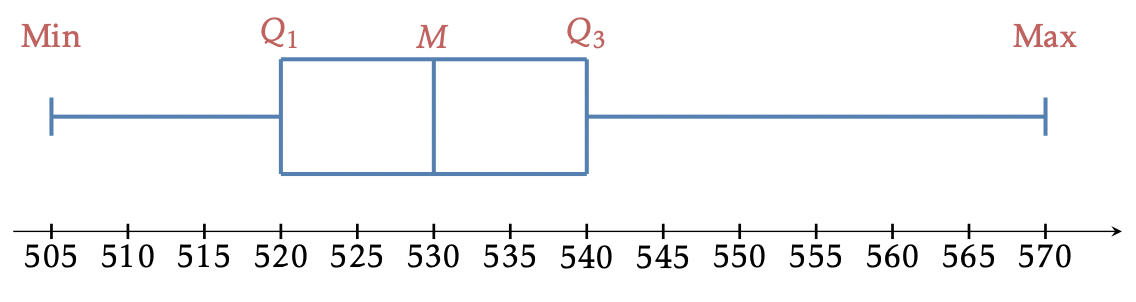
\includegraphics[scale=0.6]{Images Exercice/Boîte}
\end{center}
\begin{enumerate}
\item Lire la valeur de la médiane puis en donner une interprétation.
\item Écrire trois phrases commençant par "Environ 50 \% des shinais ont une masse comprise entre ..."
\item Calculer l'écart interquartiles.
\item Pour être homologué, la masse d'un shinai doit dépasser 510 g. \\Que penser de la production de Kumamoto?
\end{enumerate}
\end{Exercice}

\begin{Exercice}%4
Voici le pourcentage de femmes dans les parlements des 23 pays les plus peuplés du monde en 2018. \\
Thaïlande : 5 \%; Nigéria : 6 \%; Iran : 6 \%; Japon : 10 \%; Congo : 11 \%; Brésil : 11 \%;
Inde : 12 \%; Egypte : 15 \%; Turquie : 15 \%; Russie 16 \%; U.S.A : 19 \%; Indonésie : 20 \%; Bangladesh : 20 \%; Pakistan : 22 \%; Chine : 25 \%; Vietnam : 27 \%; Philippines :
29 \%; Allemagne : 31 \%; Royaume-Uni : 32 \%; Italie : 35 \%; Éthiopie : 39 \%; France : 39 \%; Mexique : 42 \%.\\
(Source: http://archive.ipu.org/wmn-f/classif.html)
\begin{enumerate}
\item Calculer la médiane Me de cette série.
\item Interpréter ce résultat en utilisant les mots : femmes - pays - parlement - moins - moitié - \%.
\item Calculer les quartiles $ Q_1 $ et $ Q_3 $.
\item Interpréter chacun de ces deux résultats.
\item Calculer l'écart interquartiles.
\end{enumerate}
\end{Exercice}

\begin{Exercice}%5
Une fabrique de céréales pour le petit-déjeuner confectionne des paquets de 300 g.
Les machines prévues pour le remplissage sont testées régulièrement.
Voici les résultats d'un test portant sur un échantillon de 997 paquets.

\begin{center}
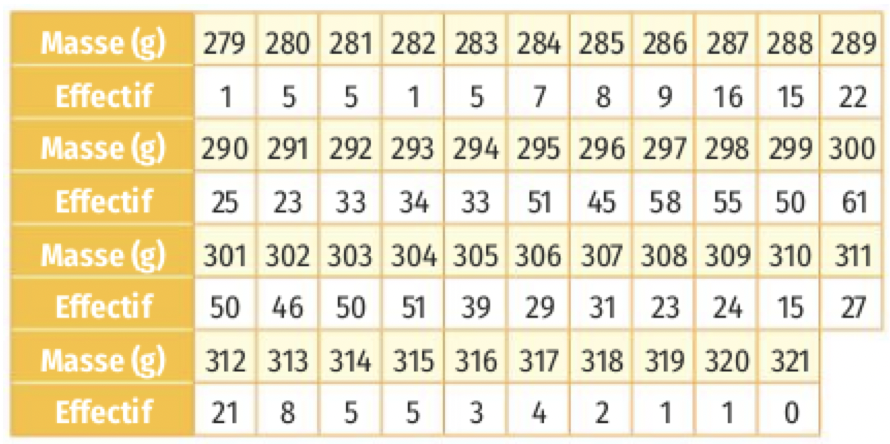
\includegraphics[scale=0.7]{Images Exercice/Stats Ex5}
\end{center}
\begin{enumerate}
\item À l'aide de la calculatrice, déterminer le minimum, la médiane, les 1er et 3e quartiles, le maximum et l'écart interquartile de cette série.
\item Tracer le diagramme en boîte de cette série.
\item Voici les critères retenus par la fabrique pour ses machines :
\begin{enumerate}
\item $ 299 \leq M \leq 301 $.
\item $ 295 \leq Q_1 $.
\item $ Q_3 \leq 305 $.
\item $ E_{Q} \in [0;9] $
\item moins de 1,5 \% des valeurs en dehors de $ [Q_1 - 1,5E_{Q}; Q_3 + 1,5E_{Q}] $.

\end{enumerate}
\noindent La machine testée réussit-elle le test?
\end{enumerate}
\end{Exercice}

\begin{Exercice} %6
Une SCOP (Société coopérative ouvrière de production) a dégagé des bénéfices cette année.
Pour l'an prochain, elle décide d'augmenter tous les salaires mensuels de 10\%, puis de les augmenter de 100 €.
Cette année le salaire moyen était de 1 700 €.
\begin{enumerate}
\item Quel sera le salaire moyen l'an prochain?
\item Estimer comment va évoluer l'écart type?
\end{enumerate}
\end{Exercice}

\newpage

\begin{Exercice} %7
Une personne compte le nombre de mail reçus chaque jour pendant un an. Les résultats sont donnés dans le tableau ci-dessous.

\begin{center}
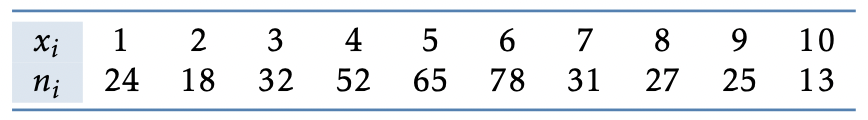
\includegraphics[scale=0.7]{Images Exercice/Stats Ex7}
\end{center}

\begin{enumerate}
\item Calculer une valeur approchée de la moyenne $ \overline{x} $ et de l'écart type $ \sigma $ de cette série.
\item Si leur effectif augmentait, donner les valeurs de $ x_i $ qui feraient :
\begin{enumerate}
\item baisser en même temps $ \overline{x} $ et $ \sigma $.
\item augmenter en même temps $ \overline{x} $ et $ \sigma $.
\end{enumerate}
\end{enumerate}
\end{Exercice}

\begin{Exercice} %8
On a représenté ci-dessous quatre cibles avec l'impact de cinq flèches tirées à l'arc.
Chaque couronne a un rayon de 1 unité.
\begin{center}
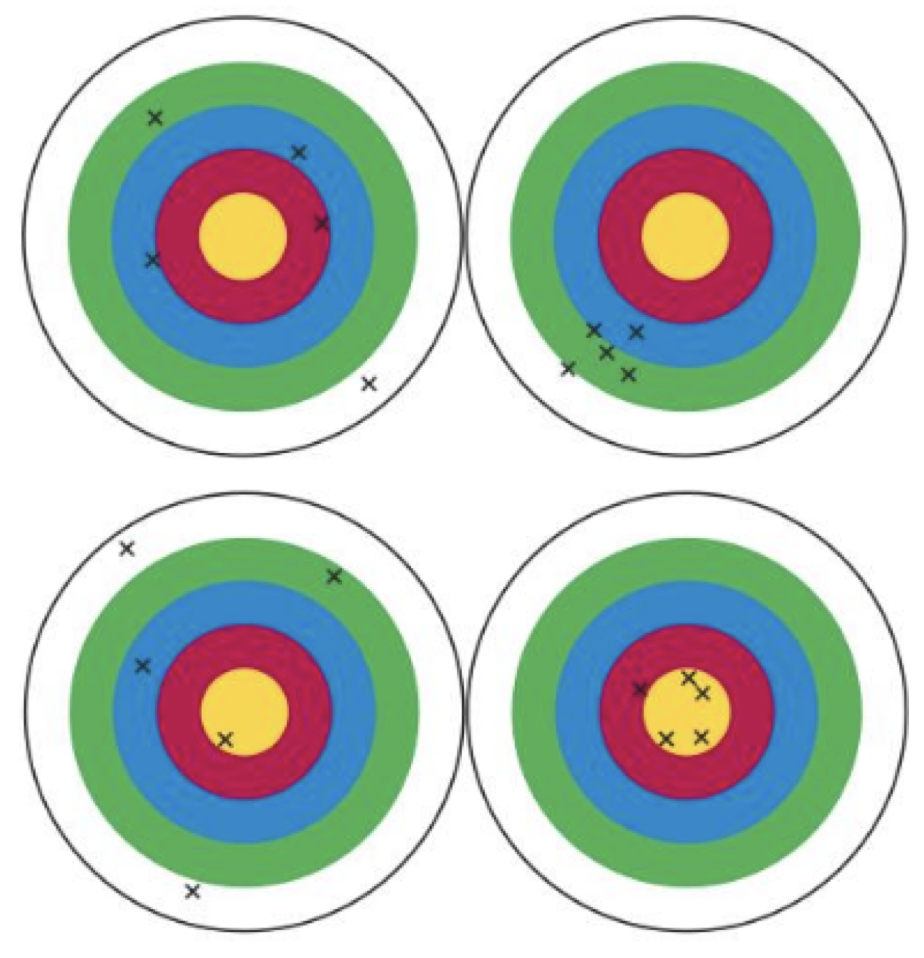
\includegraphics[scale=0.5]{Images Exercice/Stat Ex8}
\end{center}
Pour chaque tireur, on considère la distance de chaque flèche au centre de la cible.
\begin{enumerate}
\item Associer chaque couple (moyenne; écart type) à chaque cible : (2,85;0,97);
(0,79;0,19); (3,33;0,55); (3,21;1,42).
\item Associer chacun des quatre tireurs à une cible : un tireur expérimenté, deux tireurs débutants et un tireur ayant mal réglé son viseur.
\end{enumerate}
\end{Exercice}

\newpage

\begin{Exercice}%9
Une société a en charge l'entretien de distributeurs automatiques.
Elle a observé durant une année le nombre d'interventions réalisées sur chacun des distributeurs.\\

\begin{minipage}[c]{0.7\linewidth}
\begin{enumerate}
\item Déterminer le nombre moyen d'interventions $ \overline{x} $, ainsi que l'écart type $ \sigma $.
\item Le responsable de la société considère qu'il faut changer les distributeurs si l'intervalle $ [\overline{x}-2\sigma;\overline{x}+2\sigma] $ contient moins de 95 \% des valeurs de la série.
Quelle va être sa décision?
\item Il s'aperçoit qu'il a oublié de compter un distributeur sur lequel on a relevé 3 pannes.
Cela change-t-il sa décision?
\end{enumerate}
\end{minipage}
\begin{minipage}[c]{0.25\linewidth}
\begin{center}
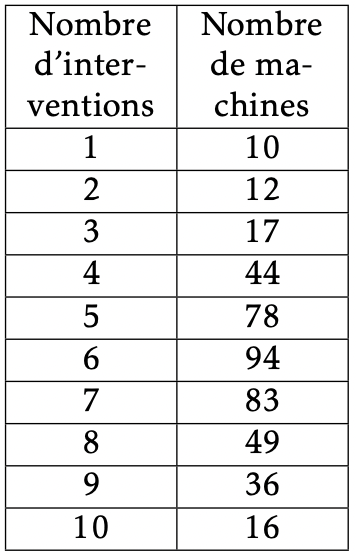
\includegraphics[scale=0.5]{Images Exercice/Stat Ex9}
\end{center}
\end{minipage}

\end{Exercice}
\vspace{-0.3cm}
\begin{Exercice}%10
Chicago et Rome sont situées à la même latitude
Voici les relevés des températures moyennes à la mi-journée des deux villes en 2017.

\begin{center}
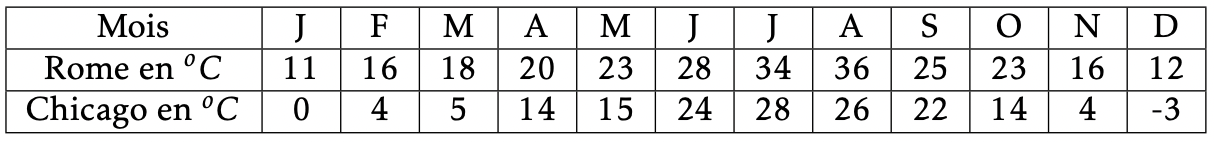
\includegraphics[scale=0.5]{Images Exercice/Stat Ex10}
\end{center}
\begin{enumerate}
\item Calculer la moyenne et l'écart-type pour chacune des deux séries afin de comparer les températures de Rome et de Chicago en 2017.
\item SVT et Géographie : Comment expliquer ces différences pour deux villes situées à la même latitude?
\end{enumerate}
\end{Exercice}
\vspace{-0.3cm}

\begin{Exercice}%11
On a résumé une série statistique dans le tableau ci-dessous.
\begin{center}
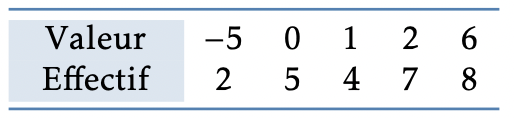
\includegraphics[scale=0.55]{Images Exercice/Stat Ex11}
\end{center}
\begin{enumerate}
\item Prévoir, sans calcul, si la moyenne de cette série sera supérieure, inférieure ou égale à la médiane? Justifier.
\item Vérifier par le calcul. Arrondir à $ 10^{-7} $
\item Déterminer les quartiles et l'écart interquartile.
\end{enumerate}
\end{Exercice}

\vspace{-0.3cm}

\begin{Exercice}%12
Les résultats d'un contrôle de vitesse en agglomération sont consignés dans le tableau ci-dessous.\\

\begin{minipage}[c]{0.35\linewidth}
\begin{center}
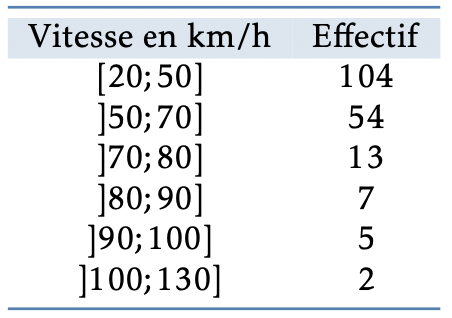
\includegraphics[scale=0.6]{Images Exercice/Stat Ex12}
\end{center}
\end{minipage}
\begin{minipage}[c]{0.60\linewidth}
\begin{enumerate}
\item On suppose que dans chaque classe, les éléments sont répartis de manière uniforme. \\
Estimer la vitesse moyenne enregistrée.
\item \begin{enumerate}[label=\alph*.]
\item En dressant la courbe des fréquences cumulées croissantes, estimer la médiane et les quartiles de cette série.
\item Pour chaque résultat, faire une phrase d'interprétation.

\end{enumerate}
\end{enumerate}
\end{minipage}

\end{Exercice}


}
